\chapter{Repository Organisation}
%================================
If you access the repository via the \trac{} browser, you should see something like figure \ref{fig:main_repository}, where the repository is organised into the usual \f{trunk}, \f{branches}, and \f{tags} subdirectories.
\begin{figure}[htb]
  \centering
  \includegraphics[scale=0.5]{graphics/main_repository.eps}
  \caption{The root of the CRTM repository organised into the typical \f{trunk}, \f{branches}, and \f{tags} subdirectories.}
  \label{fig:main_repository}
\end{figure}

\section{\f{trunk} subdirectory}
%------------------------------------
Mainline development of the CRTM is done in the trunk. Navigating the \href{https://svnemc.ncep.noaa.gov/projects/crtm/trunk}{\f{trunk}} link of the web page shown in figure \ref{fig:main_repository}, displays the various categories of the CRTM repository as shown in figure \ref{fig:trunk_repository}. 
\begin{figure}[htb]
  \centering
  \includegraphics[scale=0.5]{graphics/trunk_repository.eps}
  \caption{The trunk of the CRTM repository, showing the various categories.}
  \label{fig:trunk_repository}
\end{figure}
A short description of the trunk subdirectories are shown in table \ref{tab:trunk_category_description}
\begin{table}[htb]
  \centering
  \begin{tabular}{p{2cm} p{12cm}}
    \hline
    \sffamily\textbf{Category} & \sffamily\textbf{Description} \\
    \hline\hline
    \f{doc}       & CRTM documentation\\
    \f{externals} & Library of third party software used in the CRTM and/or support software\\
    \f{fix}       & Coefficient datafiles used by the CRTM.\\
    \f{scripts}   & Hierarchy of script software, for various languages, used in CRTM build, testing, visualisation, etc.\\
    \f{src}       & Main CRTM Fortran95 source code directory. Contains the core CRTM modules as well as support software.\\
    \f{test}      & CRTM testing. Contains code to perform unit and component test on the CRTM.\\
    \f{validation} & CRTM validation. Contains code to validate the CRTM and components.\\
    \f{web}       & The CRTM webpage source.\\
    \hline
  \end{tabular}
  \caption{Description of the contents of the CRTM repository trunk categories.}
  \label{tab:trunk_category_description}
\end{table}

As indicated, the \f{src} subdirectory is the one that contains the actual CRTM source code. This and the \f{fix} directory, which contains all of the spectral, transmittance, aerosol, cloud, and surface emissivity coefficient datafiles, are the two main parts of the CRTM repository.


\section{\f{branches} subdirectory}
%---------------------------------------
Development independent of the main CRTM trunk is done in the branches subdirectory. The current state of the CRTM \f{branches} subdirectory is shown in figure \ref{fig:branches_repository}. Note that previously, only the \f{src} directory was branched -- see figure \ref{fig:branches_src_repository} for a list of those branches. This branching methodology has been superceded by a branch of the entire trunk so that any branch is a completely self-contained copy of the CRTM trunk.

There are two types of branches in the CRTM:
\begin{enumerate}
  \item Experimental developmental branches where wholescale changes to the CRTM may result in instability. The naming convention is \f{EXP-}\textit{desc} where \textit{desc} is a short description of the experiment. For example, a branch named \f{EXP-Visible} has been created to incorporate visible sensors in the CRTM. 
  \item Code release branches where the code is tested and ``tweaked'' prior to a release. The naming convention here is \f{RB-}\textit{rel} where \textit{rel} is the planned release version number.
\end{enumerate}

\begin{figure}[htb]
  \centering
  \includegraphics[scale=0.5]{graphics/branches_repository.eps}
  \caption{Snapshot of the \f{branches} subdirectory of the CRTM repository, showing the current branches.}
  \label{fig:branches_repository}
\end{figure}


\begin{figure}[htb]
  \centering
  \includegraphics[scale=0.5]{graphics/branches_src_repository.eps}
  \caption{Snapshot of the \f{branches/src} subdirectory of the CRTM repository, showing the current branches. Note that this strategy of only branching the \f{src} directory has been replaced by complete \f{trunk} branches as shown in figure \ref{fig:branches_repository}.}
  \label{fig:branches_src_repository}
\end{figure}


\section{\f{tags} subdirectory}
%-----------------------------------
If a snapshot of development is wanted, or if development has been completed on a trunk or branch revision, a copy is made and placed in the \f{tags} subdirectory. Note that there is no development in a tag directory - it is strictly a snapshot of a trunk or branch revision.

There are three tag naming conventions in current use:
\begin{enumerate}
  \item For official software releases, \f{REL-}\textit{rel}; where \textit{rel} is the software relase number. For example, the current official CRTM release has the tag \f{REL-1.2.1}.
  \item For pre-release snapshots, \f{REL-}\textit{rel}\f{\_}\textit{stage}\f{.}\textit{YYYY-MM-DD}; where \textit{stage} is the release stage, typically \f{alpha} or \f{beta}, and \textit{YYYY-MM-DD} is the date on which the tag was created. Note that the current release number is no longer associated with a tag. An example is \f{REL-1.2.1\_beta.2009-05-01}. 
  \item For experimental branch snapshots, \f{EXP-}\textit{desc}\f{.}\textit{YYYY-MM-DD}; where \textit{desc} is a short description of the experimental branch. An example of this is \f{EXP-Visible.2009-05-07}.
\end{enumerate}

The current state of the CRTM \f{tags} subdirectory is shown in figure \ref{fig:tags_repository}. As with the \f{branches} directory, previously only the \f{src} directory was tagged -- see figure \ref{fig:tags_src_repository} for a list of those tags. This tagging methodology has been superceded by a tag of the entire trunk so that any tag is a completely self-contained copy of the CRTM trunk or branch.

\begin{figure}[htb]
  \centering
  \includegraphics[scale=0.5]{graphics/tags_repository.eps}
  \caption{Snapshot of the \f{tags} subdirectory of the CRTM repository, showing some current tags.}
  \label{fig:tags_repository}
\end{figure}

\begin{figure}[htb]
  \centering
  \includegraphics[scale=0.5]{graphics/tags_src_repository.eps}
  \caption{Snapshot of the \f{tags/src} subdirectory of the CRTM repository, showing some current tags. Note that this strategy of only tagging the \f{src} directory has been replaced by complete \f{trunk} or \r{branches} tags as shown in figure \ref{fig:tags_repository}.}
  \label{fig:tags_src_repository}
\end{figure}
